% Options for packages loaded elsewhere
\PassOptionsToPackage{unicode}{hyperref}
\PassOptionsToPackage{hyphens}{url}
\PassOptionsToPackage{dvipsnames,svgnames,x11names}{xcolor}
%
\documentclass[
  12pt]{article}

\usepackage{amsmath,amssymb}
\usepackage{iftex}
\ifPDFTeX
  \usepackage[T1]{fontenc}
  \usepackage[utf8]{inputenc}
  \usepackage{textcomp} % provide euro and other symbols
\else % if luatex or xetex
  \usepackage{unicode-math}
  \defaultfontfeatures{Scale=MatchLowercase}
  \defaultfontfeatures[\rmfamily]{Ligatures=TeX,Scale=1}
\fi
\usepackage{lmodern}
\ifPDFTeX\else  
    % xetex/luatex font selection
\fi
% Use upquote if available, for straight quotes in verbatim environments
\IfFileExists{upquote.sty}{\usepackage{upquote}}{}
\IfFileExists{microtype.sty}{% use microtype if available
  \usepackage[]{microtype}
  \UseMicrotypeSet[protrusion]{basicmath} % disable protrusion for tt fonts
}{}
\makeatletter
\@ifundefined{KOMAClassName}{% if non-KOMA class
  \IfFileExists{parskip.sty}{%
    \usepackage{parskip}
  }{% else
    \setlength{\parindent}{0pt}
    \setlength{\parskip}{6pt plus 2pt minus 1pt}}
}{% if KOMA class
  \KOMAoptions{parskip=half}}
\makeatother
\usepackage{xcolor}
\setlength{\emergencystretch}{3em} % prevent overfull lines
\setcounter{secnumdepth}{5}
% Make \paragraph and \subparagraph free-standing
\makeatletter
\ifx\paragraph\undefined\else
  \let\oldparagraph\paragraph
  \renewcommand{\paragraph}{
    \@ifstar
      \xxxParagraphStar
      \xxxParagraphNoStar
  }
  \newcommand{\xxxParagraphStar}[1]{\oldparagraph*{#1}\mbox{}}
  \newcommand{\xxxParagraphNoStar}[1]{\oldparagraph{#1}\mbox{}}
\fi
\ifx\subparagraph\undefined\else
  \let\oldsubparagraph\subparagraph
  \renewcommand{\subparagraph}{
    \@ifstar
      \xxxSubParagraphStar
      \xxxSubParagraphNoStar
  }
  \newcommand{\xxxSubParagraphStar}[1]{\oldsubparagraph*{#1}\mbox{}}
  \newcommand{\xxxSubParagraphNoStar}[1]{\oldsubparagraph{#1}\mbox{}}
\fi
\makeatother


\providecommand{\tightlist}{%
  \setlength{\itemsep}{0pt}\setlength{\parskip}{0pt}}\usepackage{longtable,booktabs,array}
\usepackage{calc} % for calculating minipage widths
% Correct order of tables after \paragraph or \subparagraph
\usepackage{etoolbox}
\makeatletter
\patchcmd\longtable{\par}{\if@noskipsec\mbox{}\fi\par}{}{}
\makeatother
% Allow footnotes in longtable head/foot
\IfFileExists{footnotehyper.sty}{\usepackage{footnotehyper}}{\usepackage{footnote}}
\makesavenoteenv{longtable}
\usepackage{graphicx}
\makeatletter
\def\maxwidth{\ifdim\Gin@nat@width>\linewidth\linewidth\else\Gin@nat@width\fi}
\def\maxheight{\ifdim\Gin@nat@height>\textheight\textheight\else\Gin@nat@height\fi}
\makeatother
% Scale images if necessary, so that they will not overflow the page
% margins by default, and it is still possible to overwrite the defaults
% using explicit options in \includegraphics[width, height, ...]{}
\setkeys{Gin}{width=\maxwidth,height=\maxheight,keepaspectratio}
% Set default figure placement to htbp
\makeatletter
\def\fps@figure{htbp}
\makeatother

\addtolength{\oddsidemargin}{-.5in}%
\addtolength{\evensidemargin}{-1in}%
\addtolength{\textwidth}{1in}%
\addtolength{\textheight}{1.7in}%
\addtolength{\topmargin}{-1in}%
\makeatletter
\@ifpackageloaded{caption}{}{\usepackage{caption}}
\AtBeginDocument{%
\ifdefined\contentsname
  \renewcommand*\contentsname{Table of contents}
\else
  \newcommand\contentsname{Table of contents}
\fi
\ifdefined\listfigurename
  \renewcommand*\listfigurename{List of Figures}
\else
  \newcommand\listfigurename{List of Figures}
\fi
\ifdefined\listtablename
  \renewcommand*\listtablename{List of Tables}
\else
  \newcommand\listtablename{List of Tables}
\fi
\ifdefined\figurename
  \renewcommand*\figurename{Figure}
\else
  \newcommand\figurename{Figure}
\fi
\ifdefined\tablename
  \renewcommand*\tablename{Table}
\else
  \newcommand\tablename{Table}
\fi
}
\@ifpackageloaded{float}{}{\usepackage{float}}
\floatstyle{ruled}
\@ifundefined{c@chapter}{\newfloat{codelisting}{h}{lop}}{\newfloat{codelisting}{h}{lop}[chapter]}
\floatname{codelisting}{Listing}
\newcommand*\listoflistings{\listof{codelisting}{List of Listings}}
\makeatother
\makeatletter
\makeatother
\makeatletter
\@ifpackageloaded{caption}{}{\usepackage{caption}}
\@ifpackageloaded{subcaption}{}{\usepackage{subcaption}}
\makeatother

\ifLuaTeX
  \usepackage{selnolig}  % disable illegal ligatures
\fi
\usepackage[]{natbib}
\bibliographystyle{agsm}
\usepackage{bookmark}

\IfFileExists{xurl.sty}{\usepackage{xurl}}{} % add URL line breaks if available
\urlstyle{same} % disable monospaced font for URLs
\hypersetup{
  pdftitle={Design-Based Variance Estimation for Latent Class Analysis of Complex Survey Data, with an Application to Institutional Trust in Mexico},
  pdfauthor={Kevin Linares},
  pdfkeywords={latent class analysis, complex survey data, replicate
variance estimation, jackknife, design effects, three-step
estimation, institutional trust},
  colorlinks=true,
  linkcolor={blue},
  filecolor={Maroon},
  citecolor={Blue},
  urlcolor={Blue},
  pdfcreator={LaTeX via pandoc}}



\begin{document}


\def\spacingset#1{\renewcommand{\baselinestretch}%
{#1}\small\normalsize} \spacingset{1}


%%%%%%%%%%%%%%%%%%%%%%%%%%%%%%%%%%%%%%%%%%%%%%%%%%%%%%%%%%%%%%%%%%%%%%%%%%%%%%

\date{July 26, 2026}
\title{\bf Design-Based Variance Estimation for Latent Class Analysis of
Complex Survey Data, with an Application to Institutional Trust in
Mexico}
\author{
Kevin Linares\\
Joint Program in Survey Methodology, University of Maryland\\
}
\maketitle

\bigskip
\bigskip
\begin{abstract}
Latent class analysis (LCA) of categorical items collected under a
stratified, clustered, weighted sample design raises a variance problem
before it raises an estimation problem. Design-weighted point estimation
is well established and available in several packages; standard errors
that respect stratification and clustering, carried without interruption
from the measurement model through to domain estimates and covariate
contrasts, are not available jointly in R. We present an integrated
pipeline organized around that gap. Parameters are estimated by
pseudo-maximum likelihood through a weighted EM algorithm and
information criteria are calibrated by weight normalization, but the
organizing commitment is that a single stratified delete-one jackknife
(JKn) replicate design generates every standard error in the analysis:
the measurement model parameters, the segment prevalences within
domains, the bias-adjusted three-step correction, and the contrasts
between domain levels. Replicate refits are warm-started and aligned to
the full-sample solution. We show that reported design effects double as
a specification check on the variance implementation, because a
covariate that is constant within a sampling unit must have a design
effect equal to the mean cluster size, and we use that identity to
validate the implementation directly. The unweighted special case is
validated to exact agreement against an independent maximum likelihood
implementation. We illustrate the methodology with thirteen
institutional trust items from the 2023 AmericasBarometer survey of
Mexico, identifying five trust segments whose composition varies sharply
with presidential approval and satisfaction with democracy. Segment
naming is drafted by a large language model operating under a certified,
frozen prompt instrument with full analyst override.
\end{abstract}

\noindent%
{\it Keywords:} latent class analysis, complex survey data, replicate
variance estimation, jackknife, design effects, three-step
estimation, institutional trust
\vfill

\newpage
\spacingset{1.9} % DON'T change the spacing!


```

Introduction

Latent class analysis identifies unobserved population subgroups from
response patterns over categorical indicators
\citep{lazarsfeld1968, goodman1974}. When the indicators come from a
complex probability sample, fitting the model and reporting honest
uncertainty about it are different problems, and the second is where the
available tools run out.

The first problem is solved. Weighting the likelihood so that the
recovered segments and their prevalences describe the target population
rather than the achieved sample is standard
\citep{patterson2002, vermunt2007, asparouhov2005}, and placing model
selection statistics on a scale consistent with that weighted objective
is understood \citep{lumley2015}. The second problem is not solved in
any integrated way. Standard errors must respect the stratification and
clustering of the design, and they must continue to do so after the
measurement model, when segment membership is related to external
variables through a bias-adjusted three-step correction whose own
variance is easy to get wrong \citep{vermunt2010, bakk2014}.

This article describes a pipeline organized around that second problem.
Its central commitment is that \textbf{one replicate design generates
every standard error in the analysis}. The same stratified
delete-one-PSU jackknife (JKn) replicate weights that produce the
interval on a conditional response probability produce the interval on a
domain prevalence, the standard error of the BCH correction, and the
standard error of a contrast between two demographic levels. Nothing is
computed under an independence assumption at any stage, and no
delta-method approximation is used that has not been checked against the
replicates.

A second contribution is diagnostic and, we think, underused. Design
effects reported against a simple random sampling benchmark do two jobs
at once. They tell the reader what the design costs, and they check the
variance implementation itself. A covariate that is constant within a
primary sampling unit has an intracluster correlation of one and
therefore a design effect equal to the mean cluster size, exactly. If
such a covariate lands there, the cluster identifier, the replicate
weights, and the variance formula are jointly correct. We exploit that
identity in Section~\ref{sec-results-design} and recommend it as routine
practice: it is a sharper validation of a design-based variance
implementation than agreement with another point estimator, because
agreement on point estimates says nothing about variance code.

No R package meets these requirements together with a path from
measurement model to labelled analytic data product. The \texttt{poLCA}
package \citep{linzer2011} fits unweighted maximum likelihood only. The
\texttt{survey} package \citep{lumley2004, lumley2010} supplies design
declaration and replication machinery but no mixture models. The closest
existing software, the \texttt{baysc} package
\citep{wu2024, wu2026joss}, fits a weighted objective within a Bayesian
pseudo-posterior \citep{savitsky2016} with a post-hoc variance
adjustment; Section~\ref{sec-baysc} discusses the relationship in
detail. Commercial options exist, notably Mplus with
\texttt{TYPE\ =\ MIXTURE\ COMPLEX} and Latent GOLD, and Stata's
\texttt{gsem} under \texttt{svy}; the contribution here is an open,
auditable implementation in R in which every estimator corresponds line
for line to documented source code.

Throughout, we refer to latent classes as segments in all user-facing
output, a terminological preference of applied audiences; the
statistical object is unchanged.

We illustrate the methodology with an analysis of institutional trust in
Mexico using the 2023 AmericasBarometer \citep{lapop2023}. Institutional
trust batteries are a natural LCA application: respondents rarely trust
or distrust all institutions uniformly, and the substantive interest
lies in the configuration of trust across institutions, which a
unidimensional scale conceals. Five segments emerge, ranging from
generalized distrust to broad confidence, with two intermediate profiles
distinguished chiefly by their treatment of the president and the armed
forces relative to representative and justice institutions.

Section~\ref{sec-appendix} documents the pipeline's operation, so that
this article also serves as reference documentation for the
implementation.

Data

The 2023 AmericasBarometer round in Mexico interviewed 1,622 voting-age
adults under a stratified, clustered design with 4 strata and 130
primary sampling units, released with base weights \citep{lapop2023}. We
analyze the thirteen-item institutional trust battery: trust in the
justice system, the electoral tribunal, the armed forces, the
legislature, the public ministry, the national police, the federal
auditor, political parties, the president, the supreme court, the
respondent's municipality, the media, and elections. Each item is
answered on a seven-point scale anchored at 1, none at all
(\emph{nada}), and 7, a lot (\emph{mucho}); intermediate points are
unlabelled. Nonresponse codes are recoded to missing during preparation,
and each item is recoded to consecutive integers over its substantive
categories, on every row of the file so that the estimation frame and
the prediction frame share one coding.

The released weights for this single-country file are effectively
constant, so the sample is self-weighting. This has a consequence worth
stating plainly at the outset: the weighted and unweighted fits nearly
coincide, and the application therefore exercises the design correction
to \emph{inference} rather than the weighting correction to \emph{point
estimates}. That is the correct emphasis for this article, whose
contribution is variance estimation, but a reader looking for evidence
that weighting changes conclusions will not find it here and should not
expect to.

Estimation uses cases complete on the thirteen trust items. Profiling
covariates may be missing without excluding a respondent from the
measurement model: conditioning the measurement model on covariate
response would introduce a selection on the very characteristics being
profiled, since item nonresponse on attitudinal batteries is not random.
Section~\ref{sec-assignment} describes how the fitted model then assigns
segment membership to item-partial respondents in the preserved full
file, subject to a minimum-information floor, and
Section~\ref{sec-domains} describes why all domain estimation runs on
that larger scored frame rather than on the estimation sample. Profiling
covariates are age category, sex, education, urban or rural residence,
and employment status. Satisfaction with democracy and evaluation of the
president's job performance are treated separately in
Section~\ref{sec-results-criterion} as criterion variables rather than
as demographics, for reasons given there.

Methods

\section{Model}\label{sec-model}

Let \(\mathbf{y}_i = (y_{i1}, \dots, y_{iJ})\) denote respondent \(i\)'s
responses to \(J\) nominal items, item \(j\) having \(C_j\) categories.
With \(K\) latent segments, prevalences \(\pi_k\), and conditional
response probabilities \(\rho_{jck} = P(y_{ij} = c \mid X_i = k)\) where
\(X_i\) denotes latent membership, the marginal probability of a
response pattern is

\begin{equation}\phantomsection\label{eq-lca}{
P(\mathbf{y}_i) \;=\; \sum_{k=1}^{K} \pi_k \prod_{j=1}^{J} \rho_{j\,y_{ij}\,k},
\qquad \sum_{k=1}^{K}\pi_k = 1, \qquad \sum_{c=1}^{C_j} \rho_{jck} = 1 .
}\end{equation}

Conditional independence of the items given segment membership, local
independence, is the load-bearing assumption;
Section~\ref{sec-diagnostics} probes where it strains and
Section~\ref{sec-assignment} exploits it for prediction under item
nonresponse. The model dimension is

\begin{equation}\phantomsection\label{eq-df}{
d_K = (K - 1) + K \sum_{j=1}^{J} (C_j - 1),
}\end{equation}

one free parameter per prevalence beyond the last and \(C_j - 1\) free
conditional probabilities per item per segment. This quantity grows
linearly in \(K\) with slope \(\sum_j (C_j-1)\), so batteries with many
response categories become expensive quickly: thirteen seven-category
items at \(K = 5\) carry 394 free parameters.

\section{Design-weighted pseudo-maximum likelihood}\label{sec-pml}

Under a complex design with base weights \(w_i\), estimation maximizes
the pseudo-log-likelihood

\begin{equation}\phantomsection\label{eq-pll}{
\ell_w(\boldsymbol\theta) \;=\; \sum_{i=1}^{n} w_i \,
\log\!\Big( \sum_{k=1}^{K} \pi_k \prod_{j=1}^{J} \rho_{j\,y_{ij}\,k} \Big),
}\end{equation}

the standard device for LCA under complex sampling
\citep{patterson2002, vermunt2007, skinner1989}. This is a
pseudo-likelihood rather than a likelihood: it is the sample-based
estimate of the census log-likelihood that would be computed if the
whole population were observed. Its maximizer is consistent for the
census parameter under standard conditions, but it is not the maximizer
of a probability model for the observed data, which is why the design
must supply the variance.

The EM algorithm \citep{dempster1977} alternates an E-step computing
posterior membership probabilities,

\begin{equation}\phantomsection\label{eq-estep}{
p_{ik} \;=\; \frac{\pi_k \prod_j \rho_{j\,y_{ij}\,k}}
{\sum_{l} \pi_l \prod_j \rho_{j\,y_{ij}\,l}},
}\end{equation}

and an M-step in which the weights enter every sufficient statistic,

\begin{equation}\phantomsection\label{eq-mstep}{
\hat\pi_k = \frac{\sum_i w_i\, p_{ik}}{\sum_i w_i}, \qquad
\hat\rho_{jck} = \frac{\sum_i w_i\, p_{ik}\, \mathbf{1}(y_{ij} = c)}
{\sum_i w_i\, p_{ik}\, \mathbf{1}(y_{ij} \text{ observed})} .
}\end{equation}

The restriction of the \(\hat\rho\) denominator to respondents who
answered item \(j\) is what makes the conditional probabilities sum to
one over \(c\) when items are partially observed; with complete cases
the restriction is vacuous and the denominator reduces to
\(\sum_i w_i p_{ik}\).

The implementation accumulates \(\log \rho_{j\,y_{ij}\,k}\) across items
and applies the log-sum-exp identity before exponentiating. With \(J\)
items this is not optional: the raw product underflows to zero for a
respondent with an improbable response pattern and
Equation~\ref{eq-estep} becomes \(0/0\). A missing item contributes zero
to the log-scale accumulation, which is exactly equivalent to dropping
it from the product in Equation~\ref{eq-lca}, and this equivalence, not
an approximation, is what licenses Equation~\ref{eq-partial} below.

Iteration stops when \(|\Delta \ell_w| < \varepsilon\,(|\ell_w| + 1)\).
During enumeration \(\varepsilon = 10^{-8}\) with at most 800 iterations
per start; the chosen model is refit at \(\varepsilon = 10^{-10}\) with
at most 5,000 iterations, matching the stopping behavior of the
reference implementation used for validation so that the comparison in
Section~\ref{sec-validation} contrasts optima rather than stopping
rules. Replicate refits (Section~\ref{sec-variance}) use the same
terminal tolerance, because the jackknife variance is a sum of squared
deviations from the full-sample estimate and systematically
under-converged replicates would enter as a bias in every one of those
deviations.

Because the pseudo-likelihood of a finite mixture can be multimodal with
near-tied optima, each candidate model is fit from many random starts
and the reported solution is the best mode found; this claim discipline
is stated rather than hidden. Starting values are generated in the main
session from a deterministic seed sequence and passed to parallel
workers as data, so no worker touches the random number generator and
results are identical under sequential and parallel execution. The
implementation asserts this at runtime by refitting the chosen model
sequentially and comparing log-likelihoods. Point estimates are
invariant to the scale of the weights.

Because the likelihood is invariant to permutation of segment labels,
any two fits must be aligned before they can be compared coordinate by
coordinate. We align a fit to a reference by minimizing total squared
distance between their response profiles over permutations, solved
exactly by the Hungarian algorithm \citep{kuhn1955, hornik2005} rather
than by heuristic matching. Alignment is applied to replicate refits
before they enter the variance, to the unweighted benchmark before
comparison, and to any comparison across \(K\). The general
label-switching problem in mixture models is harder than this
\citep{stephens2000, papastamoulis2014}; warm starting from a common
solution means alignment here confirms a correspondence rather than
discovering one.

\section{Model selection}\label{sec-selection}

Information criteria compare the maximized log-likelihood against a
sample-size penalty, and the two must sit on the same scale. Base
weights rarely sum to \(n\); because \(\ell_w\) is linear in the
weights, multiplying it by \(n / \sum_i w_i\) is exactly equivalent to
fitting with weights rescaled to sum to \(n\), leaving point estimates
untouched and calibrating only model selection. With
\(\ell^{*}_w = \ell_w \cdot n / \sum_i w_i\) we report

\begin{equation}\phantomsection\label{eq-ic}{
\mathrm{AIC} = -2\ell^{*}_w + 2 d_K, \qquad
\mathrm{BIC} = -2\ell^{*}_w + d_K \log n .
}\end{equation}

Rescaling fixes the numerator and leaves the denominator. On a design
with variable weights the information in \(n\) observations is less than
the information in \(n\) independent observations, so \(\log n\)
overstates the evidentiary hurdle. We therefore report a second
criterion using the Kish effective sample size \citep{kish1965},

\begin{equation}\phantomsection\label{eq-biceff}{
n_{\mathrm{eff}} = \frac{\big(\sum_i w_i\big)^2}{\sum_i w_i^2},
\qquad
\mathrm{BIC}_{\mathrm{eff}} = -2\ell^{*}_w + d_K \log n_{\mathrm{eff}} ,
}\end{equation}

alongside the first, so that a disagreement between them is visible
rather than hidden by a choice of default. \citet{lumley2015} develop
the general design-based treatment of information criteria and should be
consulted for the fuller account; Equation~\ref{eq-biceff} is a
practical device that makes weight variation visible in the selection
statistics, not a claim to have implemented their criterion. Note that
\(n_{\mathrm{eff}} = n\) exactly when weights are constant, so the two
criteria coincide for a self-weighting file, and the correction responds
to weight variation rather than to clustering. In the present
application they are identical for that reason, and the gap between them
should in general be read as a lower bound on the design's cost.

We report alongside these the relative entropy of the posterior
classification, on the weighted scale,

\begin{equation}\phantomsection\label{eq-entropy}{
R^2_E \;=\; 1 - \frac{-\sum_{i} w_i \sum_{k} p_{ik} \log p_{ik}}
{\big(\sum_i w_i\big) \log K},
}\end{equation}

which indexes classification sharpness \citep{ramaswamy1993}. The
numerator is the weighted average posterior uncertainty and the
denominator its maximum, attained when every posterior is uniform over
the \(K\) segments, so \(R^2_E\) runs from zero at no classification
information to one at perfect separation. Weighting is not cosmetic: an
unweighted entropy would describe the achieved sample's classification
sharpness while every other quantity describes the population, and
\(R^2_E\) is the value that justifies or fails to justify holding the
measurement model fixed in Section~\ref{sec-bch}. For a self-weighting
file the two coincide.

The bootstrapped likelihood ratio test, often recommended for class
enumeration under simple random sampling \citep{nylund2007}, is
deliberately omitted: its parametric bootstrap draws new samples of
independent observations from the fitted model, which is not the process
that generated a stratified clustered sample, matching the equivalent
restriction imposed by Mplus under complex-design analysis. Nothing is
gained by reporting a p-value whose null distribution is known to be
wrong.

The number of segments is never selected automatically. The analyst
chooses \(K\) by iterating over these statistics and the diagnostics of
Section~\ref{sec-diagnostics}, and fixes it in configuration;
Section~\ref{sec-enumeration} reports that reasoning for the present
application.

\section{Replicate variance estimation}\label{sec-variance}

All uncertainty statements come from stratified delete-one-PSU jackknife
replication \citep{wolter2007, rust1996, lumley2004}. With \(n_h\) PSUs
in stratum \(h\), deleting PSU \(j\) of stratum \(h\) and reweighting
its stratum-mates by \(n_h/(n_h - 1)\) yields the replicate estimate
\(\hat\theta_{(hj)}\), and

\begin{equation}\phantomsection\label{eq-jkn}{
\widehat{V}(\hat\theta) \;=\; \sum_{h} \frac{n_h - 1}{n_h}
\sum_{j=1}^{n_h} \big( \hat\theta_{(hj)} - \hat\theta \big)^2 .
}\end{equation}

For a vector-valued estimator the same expression with the square
replaced by an outer product gives the full covariance matrix,

\begin{equation}\phantomsection\label{eq-jknmat}{
\widehat{\mathbf{V}}(\hat{\boldsymbol\theta}) \;=\; \sum_{h} \frac{n_h - 1}{n_h}
\sum_{j=1}^{n_h} \big( \hat{\boldsymbol\theta}_{(hj)} - \hat{\boldsymbol\theta} \big)
\big( \hat{\boldsymbol\theta}_{(hj)} - \hat{\boldsymbol\theta} \big)^{\top},
}\end{equation}

whose off-diagonal entries are what make the contrasts of
Section~\ref{sec-contrasts} possible without a further derivation.

It is worth being precise about why replication rather than
linearization, since a pseudo-likelihood does admit a sandwich variance
\citep{binder1983} and that is what Mplus and Stata compute. We choose
replication for three reasons specific to this problem. First, the
parameter vector is large, 394 free parameters in the present
application, and many sit near the boundary; the linearized sandwich
requires inverting an information matrix of that dimension, and the
numerical difficulties of doing so in sparse high-dimensional latent
class settings are documented \citep{patterson2002, wu2024}. Second,
replication propagates to new statistics without rederivation: once the
replicate weights exist, the classification error matrix of
Section~\ref{sec-bch} and the contrasts of Section~\ref{sec-contrasts}
inherit design-based variance by recomputation, where linearization
would require a fresh delta-method derivation at each stage. Third,
replication makes the design specification auditable, as
Section~\ref{sec-deff} explains.

Each replicate refits the weighted EM on the replicate weights,
warm-started from the full-sample solution and aligned to it, so the
resulting variance is within-mode by construction: it carries design
variance, not uncertainty about mode selection.

A stratum containing a single PSU cannot receive the \(n_h/(n_h-1)\)
scaling. The \texttt{survey.lonely.psu} option governs linearization
variance and does not change how replicate weights are constructed, so a
singleton stratum would contribute no variance and the resulting
standard errors would be anticonservative in exactly the strata where
the data are thinnest. The implementation therefore treats singleton
strata as a hard stop, and performs the check on the analysis frame
rather than the source file, because case exclusions can create
singletons that the released data do not have.

Confidence intervals for every probability, the prevalences \(\pi_k\)
and the conditional probabilities \(\rho_{jck}\), are formed on the
logit scale with the delta-method standard error

\begin{equation}\phantomsection\label{eq-logitse}{
\mathrm{se}_{\mathrm{logit}}(\hat p) = \frac{\mathrm{se}(\hat p)}{\hat p (1 - \hat p)},
}\end{equation}

which follows from
\(\mathrm{d}\,\mathrm{logit}(p)/\mathrm{d}p = 1/\{p(1-p)\}\), and
back-transformed, which keeps intervals inside \((0,1)\) without
truncation and improves coverage for probabilities near the boundary.
The critical value is \(t_{0.975, \nu}\) with \(\nu\) the design degrees
of freedom, the number of PSUs minus the number of strata, here
\(130 - 4 = 126\), rather than the normal 1.96. Cells estimated within
\(10^{-3}\) of the boundary have no meaningful logit-scale standard
error and instead receive Wald intervals truncated to \([0, 1]\),
flagged as such in the delivered tables. The same construction serves
the domain estimates of Section~\ref{sec-domains}, so one interval
method runs through the entire pipeline.

\section{Design effects as a specification check}\label{sec-deff}

For any estimate the design effect is the ratio of the design-based
variance to the variance a simple random sample of the same size would
give,
\(\mathrm{deff} = \widehat V_{\mathrm{design}} / \widehat V_{\mathrm{SRS}}\),
and the effective sample size is \(n/\mathrm{deff}\). Under equal
cluster sizes \(m\) and intracluster correlation \(\rho\), the classical
approximation is

\begin{equation}\phantomsection\label{eq-deff}{
\mathrm{deff} \;\approx\; 1 + (m - 1)\rho .
}\end{equation}

We report design effects for every profiling variable against both the
full design and a clustering-only design that drops the strata, and read
three patterns from them.

First, and this is the specification check, \textbf{a variable that is
constant within a cluster has \(\rho = 1\) and therefore
\(\mathrm{deff} = m\) exactly}. Any covariate measured at the cluster
level rather than the respondent level, such as urbanicity in an area
sample, must land at the mean cluster size. If it does, the cluster
identifier, the replicate weights, and the variance formula are jointly
correct. This is a stronger check on variance code than agreement with
an independent point estimator, which validates estimation and says
nothing about variance.

Second, a design effect below one means variance smaller than random
sampling would produce, which requires within-cluster composition to be
controlled rather than sampled. That is the signature of a quota imposed
at the final selection stage: if interviewers fill a fixed number of
respondents in a category per sampling point, between-cluster variance
for that category is suppressed and the intracluster correlation in
Equation~\ref{eq-deff} goes negative. Precision on such variables is a
fieldwork artifact rather than sampling information.

Third, if the full-design and clustering-only design effects agree,
stratification is contributing nothing and clustering accounts for the
entire departure from simple random sampling.

\section{Model-fit diagnostics}\label{sec-diagnostics}

Item discrimination summarizes how much item \(j\) separates the
segments as the mean, over segment pairs, of the total variation
distance between their conditional response distributions:

\begin{equation}\phantomsection\label{eq-discrim}{
D_j \;=\; \frac{2}{K(K-1)} \sum_{k < l} \frac{1}{2} \sum_{c=1}^{C_j}
\big| \rho_{jck} - \rho_{jcl} \big| .
}\end{equation}

The inner expression is total variation distance between two discrete
distributions, bounded in \([0,1]\) and equal to the largest difference
in probability the two assign to any event; the leading factor is the
reciprocal of the number of pairs, \(K(K-1)/2\), so \(D_j\) is a mean of
quantities each in \([0,1]\) and is itself in \([0,1]\). \(D_j = 0\)
means every segment answers item \(j\) identically, a removal candidate
for a sensitivity refit; values near one indicate sharp separation.

Discrimination is an effect size; a companion screen asks whether each
item earns its class-dependent parameters by BIC. For item \(j\), the
fitted model is compared on the same respondents against a restricted
model in which item \(j\) is made class-independent. Under local
independence the restricted model factorizes into an LCA on the
remaining items times item \(j\)'s weighted marginal, so its
pseudo-log-likelihood is available without a constrained refit as
\(\ell_{-j} + \ell_j^{\mathrm{marg}}\), its dimension is
\(d_K^{(-j)} + (C_j - 1)\), and its BIC is directly comparable to the
full model's. We report
\(\Delta\mathrm{BIC}_j = \mathrm{BIC}_{\mathrm{restricted}} - \mathrm{BIC}_{\mathrm{full}}\);
a negative value means BIC prefers dropping item \(j\)'s class
dependence. This is a ranking under a pseudo-likelihood and not a Bayes
factor, so the conventional interpretive thresholds for BIC differences
do not apply and we do not quote them.

Local independence is probed pairwise. For items \(a, b\), let
\(\widehat{P}_{ab}(c,d)\) be the design-weighted observed proportion of
the joint response \((c,d)\) and let

\begin{equation}\phantomsection\label{eq-implied}{
\Pi_{ab} = \boldsymbol\rho_a \operatorname{diag}(\boldsymbol\pi)\, \boldsymbol\rho_b^{\top}
}\end{equation}

be the model-implied joint distribution, where \(\boldsymbol\rho_a\) is
the \(C_a \times K\) matrix of conditional probabilities for item \(a\).
Equation~\ref{eq-implied} is the model's own statement about the pair:
condition on segment, multiply the two conditional distributions because
the model asserts independence given segment, and average over segments
weighted by prevalence. We report the total variation distance between
observed and implied,

\begin{equation}\phantomsection\label{eq-bvr}{
\mathrm{BVR}_{ab} \;=\; \tfrac{1}{2} \sum_{c,d}
\big| \widehat{P}_{ab}(c,d) - \Pi_{ab}(c,d) \big| .
}\end{equation}

This departs from the Pearson-type statistic conventionally reported,
and deliberately. \citet{oberski2013} showed that the Pearson
statistic's null distribution is already not chi-square for unweighted
binary data, recommending bootstrap calibration; under design weighting
and a pseudo-likelihood on a clustered sample no reference distribution
is valid at all. A statistic with no null distribution is an effect
size, and an effect size should sit on an interpretable scale.
Equation~\ref{eq-bvr} is bounded in \([0,1]\), is exactly zero under
perfect local independence, reads as the largest probability discrepancy
over any event in the two-way table, and shares its scale with
Equation~\ref{eq-discrim}. It also removes a numerical failure of the
Pearson form, which divides by the model-implied cell probability and so
can be dominated by a single near-empty corner of a large table. Large
and persistent values argue for item removal, merging, or \(K+1\).

\section{Validation against an independent
implementation}\label{sec-validation}

At unit weights, Equation~\ref{eq-pll} reduces to the ordinary
log-likelihood, so the weighted EM and \texttt{poLCA} \citep{linzer2011}
maximize the same function and must agree up to optimizer tolerance and
mode selection. The pipeline enforces this as a runtime check. The
unit-weight EM solution is obtained from the same multi-start protocol
plus one additional candidate warm-started at the \texttt{poLCA}
solution itself; since both maximize the identical function, whichever
basin attains the higher log-likelihood is retained. The retained
solution is aligned to \texttt{poLCA} by Hungarian matching, and maximum
absolute gaps in prevalences and conditional probabilities are frozen to
disk with a single pass or fail verdict at a 0.005 threshold on both
gaps, printed identically in every downstream document. Where a gap
appears, comparison of the two log-likelihoods separates flat-ridge
drift under the stopping rule, an inferior \texttt{poLCA} mode, and an
inferior EM mode calling for more starts.

This check validates estimation. It says nothing about the variance
implementation, which is why Section~\ref{sec-deff} exists.

\section{\texorpdfstring{Relationship to
\texttt{baysc}}{Relationship to baysc}}\label{sec-baysc}

The \texttt{baysc} package \citep{wu2024, wu2026joss} implements
weighted overfitted latent class analysis in a Bayesian pseudo-posterior
\citep{savitsky2016} with a post-hoc variance adjustment. It differs
from the present pipeline in three respects that matter for choosing
between them. It selects the number of classes through an overfitted
mixture with a sparsity-inducing prior, where we require the analyst to
fix \(K\). It obtains uncertainty from an adjusted posterior rather than
from replicate weights. And being Bayesian, it propagates classification
uncertainty through the posterior draws automatically, which makes a
BCH-style correction unnecessary within that framework rather than
merely optional.

The two are complements rather than competitors, and the natural
comparison is not which is correct but whether a frequentist
replicate-variance implementation and a Bayesian variance-adjusted one
agree on the same data. We note one practical consideration bearing on
availability: \texttt{baysc} is distributed through GitHub and requires
a C++ and Fortran toolchain to build, which places it outside what can
be installed in some restricted analytic environments, including
public-sector settings limited to CRAN. Where that constraint binds, a
frequentist implementation with base survey dependencies remains the
available option.

\section{Segment assignment under partial
response}\label{sec-assignment}

Membership is assigned from the posterior evaluated at the fitted
parameters. Local independence makes assignment exact rather than
approximate for item-partial respondents: a missing item drops out of
the within-segment product, so for respondent \(i\) with answered item
set \(A_i\),

\begin{equation}\phantomsection\label{eq-partial}{
p_{ik}^{\mathrm{obs}} \;=\;
\frac{\pi_k \prod_{j \in A_i} \rho_{j\,y_{ij}\,k}}
{\sum_l \pi_l \prod_{j \in A_i} \rho_{j\,y_{ij}\,l}},
}\end{equation}

and the assigned segment is \(\arg\max_k p_{ik}^{\mathrm{obs}}\). This
is the exact posterior given what respondent \(i\) answered, under the
model and under ignorability of the missingness pattern given segment.
An information floor \(m^{*}\), configured at seven of the thirteen
items here, is enforced: respondents answering fewer than \(m^{*}\)
items receive no assignment rather than a weakly informed one. We report
mean maximum posterior by number of items answered so that the floor can
be set from evidence rather than convention.

\section{Domain estimation}\label{sec-domains}

Scoring precedes domain estimation, and all domain estimates run on the
scored frame rather than the estimation sample. This follows the logic
of three-step latent class analysis, in which the assignment step covers
every respondent it validly can, and it matters substantively: item
nonresponse on an attitude battery correlates with education, age, and
other characteristics of interest, so restricting domain estimation to
complete responders introduces a selection into the composition being
estimated. The replicate design is rebuilt on the scored frame and the
singleton stratum check is repeated there.

The primary domain estimator is the design-weighted proportion of domain
\(d\) assigned to segment \(k\),

\begin{equation}\phantomsection\label{eq-domdesign}{
\hat p_{dk} \;=\; \frac{\sum_{i \in d} w_i \, \mathbf{1}(\hat X_i = k)}
{\sum_{i \in d} w_i},
}\end{equation}

with variance from the JKn replicates. Rows sum to one across segments
by construction.

\subsection{The BCH correction}\label{sec-bch}

Cross-classifying modal assignments against external variables
understates segment differences, because assignment error attenuates
composition toward the marginal \citep{bolck2004}. Writing
\(W_i = \arg\max_k p_{ik}\) for the modal assignment, treated as an
error-prone measurement of true membership \(X_i\), define the
design-weighted classification error matrix

\begin{equation}\phantomsection\label{eq-bchD}{
D_{ks} \;=\; \widehat{P}(W = s \mid X = k) \;=\;
\frac{\sum_i w_i\, p_{ik}\, \mathbf{1}(W_i = s)}{\sum_i w_i\, p_{ik}},
}\end{equation}

the weighted posterior mass of true segment \(k\) landing in assigned
segment \(s\); rows of \(\mathbf{D}\) sum to one. The correction
replaces each respondent's hard assignment with
\(\mathbf{u}_i = \mathbf{e}_{W_i}^{\top} \mathbf{D}^{-1}\), row \(W_i\)
of \(\mathbf{D}^{-1}\), and the corrected prevalence of segment \(k\)
within domain \(d\) is

\begin{equation}\phantomsection\label{eq-bchdom}{
\hat p^{\mathrm{BCH}}_{dk} \;=\; \frac{\sum_{i \in d} w_i\, u_{ik}}{\sum_{i \in d} w_i}.
}\end{equation}

The correction works because, for a respondent whose true membership is
\(m\),

\begin{equation}\phantomsection\label{eq-bchunbiased}{
\mathbb{E}\big[u_{ik} \mid X_i = m\big]
= \sum_{s} P(W = s \mid X = m)\,\big(\mathbf{D}^{-1}\big)_{sk}
= \big(\mathbf{D}\mathbf{D}^{-1}\big)_{mk} = \mathbf{1}(m = k),
}\end{equation}

so \(u_{ik}\) is unbiased for the indicator of true membership and its
weighted mean within a domain estimates \(P(X = k \mid d)\) rather than
\(P(W = k \mid d)\). Two consequences follow immediately from
Equation~\ref{eq-bchunbiased}. Entries of \(\mathbf{u}_i\) can be
negative, so individual cell estimates can fall slightly outside
\([0,1]\); this is a documented property of the method, not an error.
And each \(\mathbf{u}_i\) sums to one, because
\(\mathbf{D}\mathbf{1} = \mathbf{1}\) implies
\(\mathbf{D}^{-1}\mathbf{1} = \mathbf{1}\) and every row of
\(\mathbf{D}^{-1}\) therefore sums to one, so within every domain the
corrected prevalences still sum to one across segments.

Variance is estimated with the same JKn replicates: the posterior matrix
and modal assignments are held fixed at the full-sample measurement
model, while \(\mathbf{D}\) and the correction weights are rebuilt
inside every replicate from the replicate weights, so the intervals
carry the design variance of the classification table and the
cross-tabulation jointly. \citet{vermunt2010} is explicit that BCH point
estimates paired with uncorrected variances yield p-values that are far
too small; recomputing inside the replicates is the direct remedy.
Holding step one fixed is the standard treatment; the resulting
understatement of variance is minor when classification is sharp
\citep{bakk2014, bakk2013}.

\subsection{Contrasts between domain levels}\label{sec-contrasts}

Overlapping intervals are not a test. Because Equation~\ref{eq-jknmat}
yields the full covariance, differences between domain levels carry
their own standard errors,

\begin{equation}\phantomsection\label{eq-contrast}{
\widehat{\mathrm{Var}}\big(\hat p_{dk} - \hat p_{d'k}\big)
= \widehat V_{dd} + \widehat V_{d'd'} - 2\widehat V_{dd'} ,
}\end{equation}

with the covariance term taken from the replicates rather than assumed
zero. We compare every level of a demographic against that variable's
reference level, within segment, on the design \(t\), with Holm
adjustment \citep{holm1979} applied within each demographic variable.

\subsection{Which estimator to report}\label{sec-whichestimator}

Two of the three choices here are not choices. Segment prevalence within
a demographic group is a descriptive population quantity, so the point
estimate is weighted; and on a stratified clustered sample the
independence standard error is wrong in an unknown direction, so the
interval is design-based. The real decision is modal versus BCH, and it
has a rule: compute the shift between the two estimators and compare it
to the standard error. When the shift is a small fraction of the
standard error the correction is inside noise and the uncorrected
estimates should be reported with the correction noted as a sensitivity
check.

The direction of the bias determines when that rule may be overridden.
Attenuation always pulls toward the marginal, so it always understates
group differences. If the claim is that groups differ, modal assignment
is conservative and a surviving difference is real. If the claim is that
groups do not differ, modal assignment is not safe, because attenuation
manufactures null results. The case for retaining the correction is
therefore that it protects null findings, not positive ones. One
counterintuitive consequence: the case for BCH weakens as sample size
falls, since standard errors grow while the classification bias does
not.

\section{LLM-assisted, analyst-controlled labeling}\label{sec-labeling}

Segment naming is a bottleneck in applied LCA reporting, and recent
evidence suggests large language models perform annotation-adjacent
tasks reliably when tightly instructed \citep{gilardi2023, ziems2024}.
The pipeline drafts segment names with a language model under a fixed
instrument: a persona and rule set instructing interpretation strictly
from the displayed conditional response probabilities and item wording,
one isolated call per segment (joint prompts empirically confused
near-neighbor segments), an optional survey-context paragraph fenced to
referent resolution only, and a collision-gated harmonization pass that
may edit labels, never descriptions. Labels follow one rule: a label
file on disk is used when present and validated against \(K\); otherwise
the model drafts once and the result is frozen to that file, which the
analyst edits to take over naming. The freeze file, not a sampling seed,
is the reproducibility mechanism, because a seed would be reproducible
only for a fixed model, endpoint, and package version.

The instrument is treated as a measurement device. A certification
harness plants a known-meaning model, including near-neighbor segments,
a deliberately diffuse segment, nonresponse-labelled items, and a
fictional survey context, and checks output format, grounding in the
displayed probabilities, hedging on diffuse profiles, persona integrity,
context-leak fencing, harmonizer properties, and adoption of the segment
terminology; any edit to the instrument obliges recertification.

Labels never re-enter estimation. They are display strings attached
after every number is computed, so a wrong label is a presentation error
and not a statistical one. Labels are drafts, verified by the analyst
against the conditional response profiles before use, and the delivered
tables carry the label file's contents, not live model output.

Results

\section{Enumeration and the choice of K}\label{sec-enumeration}

Table~\ref{tbl-enum} reports the weighted fit statistics, each candidate
fit from seeded random starts; all converged. Figure~\ref{fig-enum}
plots weighted BIC and relative entropy.

\begin{longtable}[]{@{}rrrrrrr@{}}

\caption{\label{tbl-enum}Weighted fit statistics by number of segments.
The log-likelihood is on the sum-to-n scale; entropy is the weighted
relative entropy of the posterior classification. BIC and BIC on the
effective sample size coincide here because the file is self-weighting.}

\tabularnewline

\toprule\noalign{}
K & logLik & df & AIC & BIC & BIC\_eff & entropy \\
\midrule\noalign{}
\endhead
\bottomrule\noalign{}
\endlastfoot
2 & -32115.8 & 157 & 64545.7 & 65375.0 & 65375.0 & 0.903 \\
3 & -30686.4 & 236 & 61844.8 & 63091.4 & 63091.4 & 0.913 \\
4 & -29945.9 & 315 & 60521.9 & 62185.7 & 62185.7 & 0.921 \\
5 & -29526.9 & 394 & 59841.8 & 61922.9 & 61922.9 & 0.908 \\
6 & -29223.8 & 473 & 59393.6 & 61892.0 & 61892.0 & 0.895 \\
7 & -29004.9 & 552 & 59113.7 & 62029.4 & 62029.4 & 0.893 \\
8 & -28855.3 & 631 & 58972.7 & 62305.6 & 62305.6 & 0.890 \\
9 & -28707.5 & 710 & 58835.1 & 62585.3 & 62585.3 & 0.887 \\
10 & -28588.4 & 789 & 58754.9 & 62922.4 & 62922.4 & 0.896 \\

\end{longtable}

\begin{figure}

\centering{

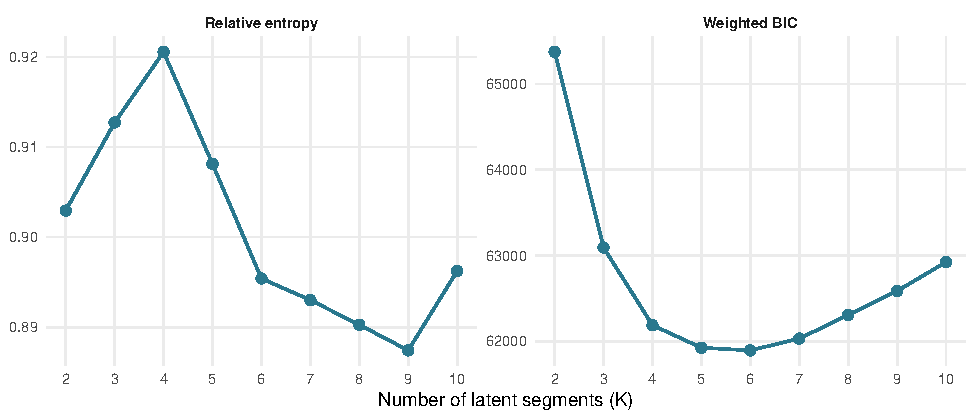
\includegraphics{survey_lca_paper_files/figure-pdf/fig-enum-1.pdf}

}

\caption{\label{fig-enum}Enumeration diagnostics across K: weighted BIC
and relative entropy.}

\end{figure}%

Weighted BIC drops steeply through \(K = 5\) (60,957.9), reaches its
minimum at \(K = 6\) (60,940.1), and rises monotonically thereafter. The
difference between the two, 17.8, is small against the preceding drops
of 226.2 (\(4 \to 5\)) and 882.9 (\(3 \to 4\)): the criterion is
effectively flat over the \(\{5, 6\}\) region. AIC continues to decline
through the whole range, its usual overextraction at large \(n\)
\citep{nylund2007}. Relative entropy peaks at \(K = 4\) (0.921) and
remains high at \(K = 5\) (0.907). Within the flat BIC region we fixed
\(K = 5\) on parsimony, classification sharpness, and interpretability:
the five-segment solution yields substantively distinct, cleanly
separated profiles (Section~\ref{sec-measurement}), whereas the marginal
BIC gain at \(K = 6\) purchases a further split at the cost of entropy.
Consistent with the flatness of the criterion, the unweighted
benchmark's own BIC minimizes at \(K = 6\) as well; enumeration under
weighting and without it point to the same region. We emphasize that
\(K\) is an analyst decision recorded in configuration, not an automated
selection, and the full enumeration evidence is reported so readers can
weigh the neighboring solution.

\section{The measurement model}\label{sec-measurement}

The chosen model converged with weighted log-likelihood \(-29{,}047.7\)
on the sum-to-\(n\) scale, relative entropy 0.907, and mean maximum
posterior probability 0.939: respondents are, on average, assigned to
their modal segment with 94 percent confidence. Table~\ref{tbl-prev}
reports the design-weighted segment prevalences with JKn intervals
alongside the unweighted benchmark, and Figure~\ref{fig-profiles}
displays the full measurement model.

\begin{longtable}[]{@{}
  >{\raggedright\arraybackslash}p{(\columnwidth - 6\tabcolsep) * \real{0.4000}}
  >{\raggedleft\arraybackslash}p{(\columnwidth - 6\tabcolsep) * \real{0.3053}}
  >{\raggedleft\arraybackslash}p{(\columnwidth - 6\tabcolsep) * \real{0.2211}}
  >{\raggedleft\arraybackslash}p{(\columnwidth - 6\tabcolsep) * \real{0.0737}}@{}}

\caption{\label{tbl-prev}Design-weighted segment prevalences with 95
percent JKn intervals (logit scale, t critical value with 126 design
degrees of freedom), the unweighted poLCA benchmark, and the weighting
gap.}

\tabularnewline

\toprule\noalign{}
\begin{minipage}[b]{\linewidth}\raggedright
Segment
\end{minipage} & \begin{minipage}[b]{\linewidth}\raggedleft
Weighted prevalence {[}95\% CI{]}
\end{minipage} & \begin{minipage}[b]{\linewidth}\raggedleft
Unweighted benchmark
\end{minipage} & \begin{minipage}[b]{\linewidth}\raggedleft
Gap
\end{minipage} \\
\midrule\noalign{}
\endhead
\bottomrule\noalign{}
\endlastfoot
S1: Guarded Political Distrust & 0.341 {[}0.300, 0.384{]} & 0.341 &
+0.000 \\
S2: Moderate, Reserved Trust & 0.207 {[}0.171, 0.249{]} & 0.207 &
+0.000 \\
S3: Widespread Institutional Distrust & 0.107 {[}0.084, 0.135{]} & 0.107
& -0.000 \\
S4: Cautious, Moderate Trust & 0.234 {[}0.192, 0.281{]} & 0.234 &
-0.000 \\
S5: High Presidential Trust & 0.112 {[}0.093, 0.134{]} & 0.112 &
+0.000 \\

\end{longtable}

\begin{figure}

\centering{

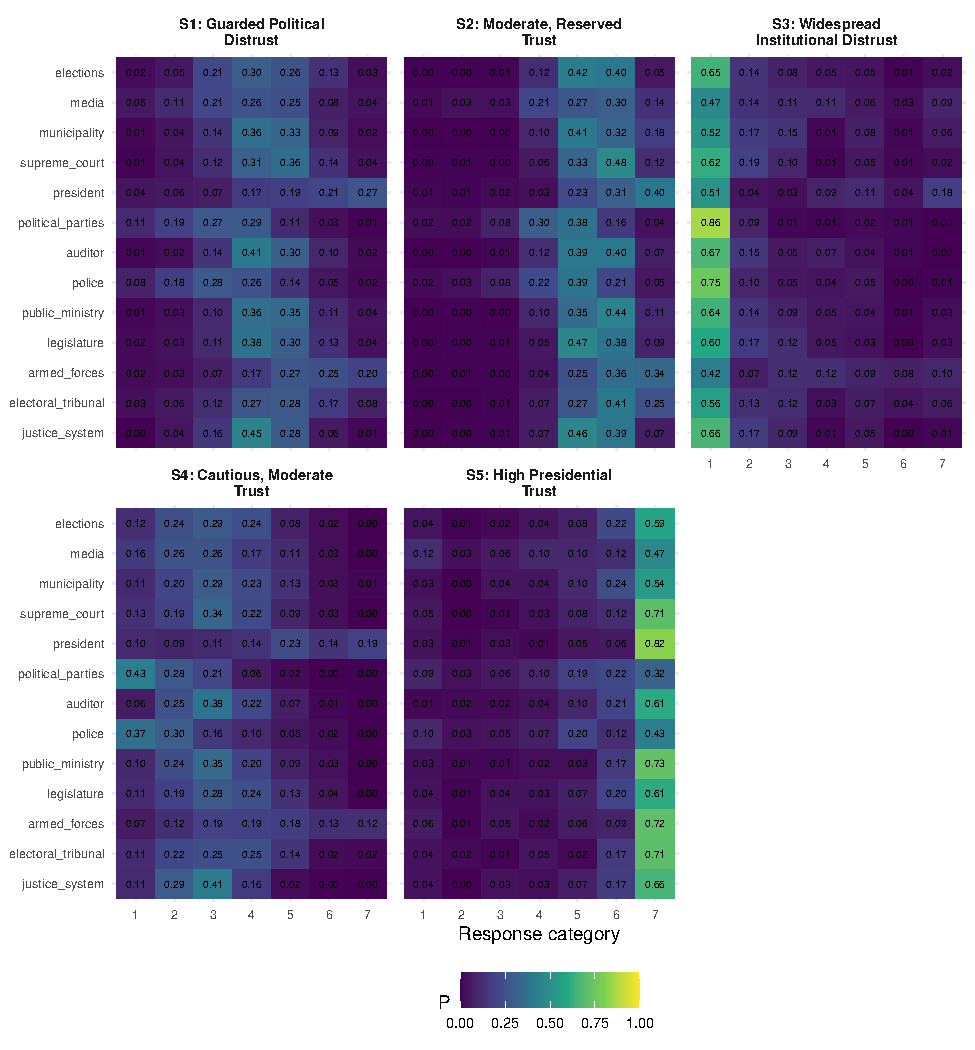
\includegraphics{survey_lca_paper_files/figure-pdf/fig-profiles-1.pdf}

}

\caption{\label{fig-profiles}Conditional response probabilities
P(response category \textbar{} segment) for all thirteen trust items.
Rows are items, columns are the seven response categories from 1 (nada)
to 7 (mucho).}

\end{figure}%

The five profiles order naturally on overall trust with two
configurational departures. Segment S5, Broad Institutional Trust
(weighted prevalence 0.208), concentrates mass on categories 5 and 6
across every institution. Segment S4, Very High National Trust (0.111),
is its extreme counterpart, with probability 0.82 of answering
\emph{mucho} on trust in the president and 0.70 or above on the public
ministry, armed forces, supreme court, and electoral tribunal. Segment
S2, Generalized Institutional Distrust (0.107), mirrors it at the other
pole, with probability 0.85 of answering \emph{nada} on political
parties and 0.76 on the national police; only the president and armed
forces draw any appreciable mass off the floor. The two largest segments
are configurational rather than uniform. Segment S1, Moderate
Institutional Trust (0.331), holds the middle categories on the justice
and audit institutions while shifting upward on the president and armed
forces. Segment S3, Presidential and Military Trust (0.242), sharpens
that asymmetry: substantial trust in the president (probability 0.21 at
\emph{mucho}, mass concentrated at 5 to 7) and the armed forces, against
firm distrust of political parties (0.41 at \emph{nada}) and the police.
The configuration, not the level, separates S1 from S3, and it is
precisely this configurational structure that a summed trust scale would
average away.

The weighted and unweighted prevalences differ by at most 0.005
(Table~\ref{tbl-prev}): the released weights for this file are nearly
constant, so weighting shifts point estimates little here. The design
still matters for inference. The interval for S1 spans 0.293 to 0.372, a
half-width of 0.0395 against the 0.0244 a simple random sample of the
same size would give, implying a design effect of about 2.6 for that
prevalence.

\section{Diagnostics}\label{sec-results-diagnostics}

\begin{figure}

\centering{

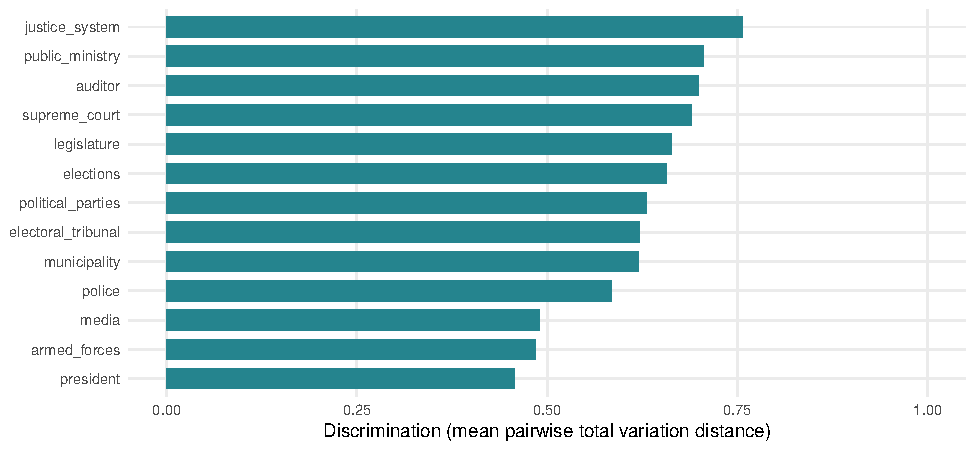
\includegraphics{survey_lca_paper_files/figure-pdf/fig-discrim-1.pdf}

}

\caption{\label{fig-discrim}Item discrimination: the mean over segment
pairs of the total variation distance between conditional response
distributions.}

\end{figure}%

Every item earns its place. Discrimination (Figure~\ref{fig-discrim})
ranges from 0.452 (president) to 0.754 (justice system); no item
approaches the region where removal would be considered. The BIC screen
of Section~\ref{sec-diagnostics} agrees: \(\Delta\mathrm{BIC}_j\) is
positive for all thirteen items, from \(+320.0\) (president) to
\(+1{,}419.3\) (justice system), so BIC prefers retaining every item's
class dependence by margins that are decisive throughout. That the
president and armed forces items discriminate least is itself
informative: they are the institutions on which otherwise different
segments agree.

\begin{longtable}[]{@{}llr@{}}

\caption{\label{tbl-bvr}Largest bivariate residuals, as total variation
distance between the design-weighted observed two-way table and the
model-implied table. Bounded in {[}0, 1{]} and zero under exact local
independence; a descriptive ranking, since no reference distribution
applies under the weighted pseudo-likelihood.}

\tabularnewline

\toprule\noalign{}
Item A & Item B & BVR \\
\midrule\noalign{}
\endhead
\bottomrule\noalign{}
\endlastfoot
public\_ministry & auditor & 0.163 \\
armed\_forces & legislature & 0.148 \\
justice\_system & supreme\_court & 0.120 \\
police & political\_parties & 0.106 \\
police & municipality & 0.104 \\

\end{longtable}

The bivariate residuals (Table~\ref{tbl-bvr}) rank the item pairs whose
residual association the five segments absorb least well. The leading
pairs are institutionally adjacent, two audit-and-prosecution bodies and
two national-state bodies, which is what a local dependence violation
from shared content looks like. Because no reference distribution is
valid here we read these as a ranked caution rather than a rejection,
one consistent with BIC's mild preference for the neighboring
six-segment solution, and we flag the leading pairs as the natural first
check in any sensitivity refit.

\section{Validation and the design
specification}\label{sec-results-design}

At unit weights the pipeline's EM and \texttt{poLCA} agree exactly: the
maximum absolute prevalence gap is 0.00000 and the maximum
conditional-probability gap is 0.00000. The implementations maximize the
same function and find the same optimum, which certifies the estimation
machinery before any weighted result is interpreted.

The variance machinery is certified separately, by
Equation~\ref{eq-deff}. The design comprises 130 PSUs with a mean
cluster size of 12.4. Urbanicity is constant within a sampling unit in
this area sample, so its intracluster correlation is one and its design
effect must equal the mean cluster size. The observed design effect for
urbanicity is 12.6 against a predicted ceiling of 12.4, agreement to two
significant figures, which confirms that the cluster identifier, the
replicate weight construction, and Equation~\ref{eq-jkn} are jointly
correct. No comparison of point estimates could establish this.

The remaining design effects are informative in their own right.
Education ranges from 1.12 to 2.37 and employment from 0.96 to 1.11, the
ordinary range for respondent-level covariates under clustering. Sex, by
contrast, returns 0.22 on both levels of a near-even split, and age
category returns 0.21 for the youngest group rising monotonically to
1.34 for the oldest. A design effect of 0.22 on a 49/51 split cannot
arise from sampling variation and is the signature described in
Section~\ref{sec-deff}: composition controlled within sampling points
rather than sampled, consistent with sex and age quotas at the final
selection stage. The standard errors on those two variables are
therefore fieldwork artifacts rather than sampling information, and we
do not read precision into them. Dropping the strata leaves every design
effect essentially unchanged, so clustering accounts for the entire
departure from simple random sampling and the four strata contribute
nothing.

\section{Assignment coverage}\label{sec-results-assignment}

Prediction under Equation~\ref{eq-partial} assigns a segment to nearly
the entire file: complete cases plus item-partial respondents meeting
the seven-item floor, with the small remainder left unassigned rather
than guessed. The delivered data product is a labelled SPSS file
carrying the numeric segment with value labels, the label text, the
posterior probabilities, the BCH correction weights, and the assignment
diagnostics, together with CSV exports of the full measurement model
with intervals, the domain composition estimates under both estimators,
and the contrasts. The posteriors and correction weights are exported
deliberately: a downstream analyst cross-tabulating the modal assignment
alone reintroduces exactly the attenuation Section~\ref{sec-bch}
removes, and the variable label on the segment column says so.

\section{Demographic composition}\label{sec-results-demographics}

\begin{longtable}[]{@{}
  >{\raggedright\arraybackslash}p{(\columnwidth - 12\tabcolsep) * \real{0.0917}}
  >{\raggedright\arraybackslash}p{(\columnwidth - 12\tabcolsep) * \real{0.1583}}
  >{\raggedright\arraybackslash}p{(\columnwidth - 12\tabcolsep) * \real{0.1500}}
  >{\raggedright\arraybackslash}p{(\columnwidth - 12\tabcolsep) * \real{0.1500}}
  >{\raggedright\arraybackslash}p{(\columnwidth - 12\tabcolsep) * \real{0.1500}}
  >{\raggedright\arraybackslash}p{(\columnwidth - 12\tabcolsep) * \real{0.1500}}
  >{\raggedright\arraybackslash}p{(\columnwidth - 12\tabcolsep) * \real{0.1500}}@{}}

\caption{\label{tbl-demo}Design-based segment prevalence within levels
of the demographic covariates, with 95 percent JKn intervals. Rows sum
to one across segments.}

\tabularnewline

\toprule\noalign{}
\begin{minipage}[b]{\linewidth}\raggedright
Variable
\end{minipage} & \begin{minipage}[b]{\linewidth}\raggedright
Level
\end{minipage} & \begin{minipage}[b]{\linewidth}\raggedright
S1
\end{minipage} & \begin{minipage}[b]{\linewidth}\raggedright
S2
\end{minipage} & \begin{minipage}[b]{\linewidth}\raggedright
S3
\end{minipage} & \begin{minipage}[b]{\linewidth}\raggedright
S4
\end{minipage} & \begin{minipage}[b]{\linewidth}\raggedright
S5
\end{minipage} \\
\midrule\noalign{}
\endhead
\bottomrule\noalign{}
\endlastfoot
age\_cat & 18-29 & 0.37 {[}0.32, 0.41{]} & 0.21 {[}0.17, 0.25{]} & 0.10
{[}0.07, 0.12{]} & 0.24 {[}0.20, 0.28{]} & 0.08 {[}0.06, 0.11{]} \\
age\_cat & 30-44 & 0.33 {[}0.28, 0.38{]} & 0.21 {[}0.16, 0.25{]} & 0.11
{[}0.08, 0.14{]} & 0.25 {[}0.21, 0.30{]} & 0.10 {[}0.07, 0.13{]} \\
age\_cat & 45-59 & 0.35 {[}0.30, 0.40{]} & 0.17 {[}0.13, 0.21{]} & 0.13
{[}0.10, 0.17{]} & 0.23 {[}0.19, 0.27{]} & 0.12 {[}0.09, 0.15{]} \\
age\_cat & 60+ & 0.33 {[}0.27, 0.38{]} & 0.24 {[}0.20, 0.29{]} & 0.12
{[}0.08, 0.16{]} & 0.16 {[}0.10, 0.21{]} & 0.16 {[}0.11, 0.20{]} \\
sex & Male & 0.34 {[}0.30, 0.37{]} & 0.22 {[}0.19, 0.26{]} & 0.11
{[}0.08, 0.13{]} & 0.22 {[}0.19, 0.26{]} & 0.11 {[}0.09, 0.13{]} \\
sex & Female & 0.36 {[}0.32, 0.39{]} & 0.18 {[}0.16, 0.21{]} & 0.12
{[}0.10, 0.14{]} & 0.23 {[}0.20, 0.26{]} & 0.11 {[}0.09, 0.13{]} \\
education & Secondary & 0.36 {[}0.33, 0.39{]} & 0.22 {[}0.19, 0.25{]} &
0.11 {[}0.09, 0.14{]} & 0.22 {[}0.19, 0.25{]} & 0.09 {[}0.07, 0.11{]} \\
education & None & 0.24 {[}0.10, 0.38{]} & 0.18 {[}0.06, 0.31{]} & 0.18
{[}0.06, 0.31{]} & 0.13 {[}0.02, 0.24{]} & 0.26 {[}0.11, 0.41{]} \\
education & Primary & 0.35 {[}0.29, 0.41{]} & 0.21 {[}0.16, 0.26{]} &
0.10 {[}0.06, 0.13{]} & 0.16 {[}0.12, 0.20{]} & 0.18 {[}0.14, 0.22{]} \\
education & Tertiary & 0.33 {[}0.27, 0.39{]} & 0.16 {[}0.11, 0.20{]} &
0.12 {[}0.08, 0.15{]} & 0.33 {[}0.27, 0.39{]} & 0.07 {[}0.04, 0.10{]} \\
urban & Urban & 0.34 {[}0.31, 0.37{]} & 0.19 {[}0.17, 0.22{]} & 0.12
{[}0.10, 0.14{]} & 0.24 {[}0.21, 0.27{]} & 0.11 {[}0.09, 0.13{]} \\
urban & Rural & 0.37 {[}0.31, 0.42{]} & 0.25 {[}0.19, 0.31{]} & 0.10
{[}0.07, 0.13{]} & 0.17 {[}0.14, 0.21{]} & 0.11 {[}0.08, 0.14{]} \\
employment & Employed & 0.35 {[}0.32, 0.38{]} & 0.20 {[}0.17, 0.23{]} &
0.13 {[}0.10, 0.15{]} & 0.23 {[}0.20, 0.26{]} & 0.10 {[}0.08, 0.12{]} \\
employment & Unemployed & 0.30 {[}0.18, 0.42{]} & 0.19 {[}0.11, 0.28{]}
& 0.12 {[}0.04, 0.21{]} & 0.29 {[}0.17, 0.40{]} & 0.10 {[}0.03,
0.16{]} \\
employment & Not in labor force & 0.36 {[}0.23, 0.49{]} & 0.18 {[}0.06,
0.30{]} & 0.08 {[}0.00, 0.16{]} & 0.30 {[}0.17, 0.43{]} & 0.08 {[}0.00,
0.16{]} \\
employment & Student & 0.39 {[}0.29, 0.49{]} & 0.25 {[}0.16, 0.34{]} &
0.08 {[}0.02, 0.15{]} & 0.19 {[}0.11, 0.27{]} & 0.08 {[}0.03, 0.14{]} \\
employment & Homemaker & 0.33 {[}0.29, 0.38{]} & 0.21 {[}0.17, 0.25{]} &
0.10 {[}0.07, 0.12{]} & 0.22 {[}0.18, 0.26{]} & 0.13 {[}0.10, 0.16{]} \\
employment & Retired & 0.37 {[}0.27, 0.47{]} & 0.17 {[}0.10, 0.24{]} &
0.10 {[}0.04, 0.15{]} & 0.19 {[}0.11, 0.27{]} & 0.17 {[}0.08, 0.26{]} \\

\end{longtable}

The demographic covariates show modest structure. Presidential and
Military Trust is more prevalent in urban areas than rural and declines
with age, while Broad Institutional Trust moves in the opposite
direction with age. Respondents with no formal education are estimated
predominantly in Very High National Trust, though this cell rests on few
observations and its interval is correspondingly wide. Differences by
sex and employment status are small, with overlapping intervals
throughout; we note that the sex comparison in particular carries the
quota-induced precision discussed in Section~\ref{sec-results-design}
and should not be read as a sharp null.

BCH-corrected estimates are reported alongside in the replication
materials. Following Section~\ref{sec-whichestimator}, we report the
uncorrected design-based estimates as primary: the shift induced by the
correction is a small fraction of the standard errors throughout, which
is what Equation~\ref{eq-bchunbiased} predicts when classification is as
sharp as relative entropy 0.907 implies. The correction is retained and
reported because it protects the null comparisons above, not because it
moves the positive ones.

\section{Criterion variables}\label{sec-results-criterion}

Presidential job approval and satisfaction with democracy are treated
separately from the demographic covariates above, and deliberately so.
They are attitudes rather than characteristics, and both are plausibly
related to institutional trust by construction, so entering them as
profiling variables would partly explain the measurement model with
itself. Their proper role is as criterion variables: they test whether
the segments behave as a trust typology should, which is a validity
question rather than a compositional one.

They do. Composition is strongly ordered in presidential approval. Among
respondents rating the president's performance very bad, Generalized
Institutional Distrust reaches 0.52 {[}0.35, 0.68{]}; among those rating
it very good, that segment falls to 0.07 while Very High National Trust
rises to 0.19 {[}0.16, 0.24{]}. Satisfaction with democracy behaves
symmetrically: Generalized Distrust is 0.34 {[}0.25, 0.45{]} among the
very dissatisfied against 0.06 among the very satisfied, while Very High
National Trust is 0.34 {[}0.25, 0.44{]} among the very satisfied against
0.05 among the very dissatisfied. Segments derived only from
institutional trust items order monotonically on two attitudes never
shown to the model, which is the behavior a valid typology should
exhibit.

The correction's behavior at sparse cells is visible in the Bad approval
row of the corrected table, where one estimate is a numerically negative
zero with a truncated interval: no respondents rating the president
badly belong, after correction, to the segment defined by near-uniform
\emph{mucho} responses that include the president item, exactly as
coherence requires and exactly as Equation~\ref{eq-bchunbiased} permits.

Discussion

The pipeline demonstrated here closes a specific gap: design-based
replicate inference for latent class analysis, carried without
interruption from the measurement model through bias-adjusted profiling
to a labelled data product, in open R code. Each component is
individually established, pseudo-maximum likelihood for LCA under
complex sampling \citep{patterson2002, vermunt2007}, weight-normalized
information criteria \citep{lumley2015}, JKn replication
\citep{wolter2007}, and the BCH correction
\citep{bolck2004, vermunt2010}; the contribution is their disciplined
integration, with the seams between components treated as first-class
design decisions rather than afterthoughts.

We would single out the design effect check of Section~\ref{sec-deff} as
the most transferable element. Validation of statistical software
overwhelmingly targets point estimates, because a second implementation
is usually available to compare against. Variance code is harder to
validate that way, since two implementations may use different variance
methods and disagree legitimately. The cluster-constant covariate
identity provides an exact, assumption-free target: the design effect
must equal the mean cluster size, and any deviation localizes the error.
It costs one extra \texttt{svydesign} call and it caught nothing here
only because the specification was already correct.

The application illustrates why the machinery matters substantively.
Institutional trust in Mexico is not unidimensional: two of the five
segments, together a third of the population, are defined by the
configuration of trust, elevated for the president and armed forces
against distrust of parties and police, rather than by its level, and
segment composition moves sharply with presidential approval. A summed
trust scale would compress exactly this structure. The near-constancy of
the released weights in this file makes the weighting correction small
for point estimates while leaving the design correction to inference
fully operative, and the design effects of
Section~\ref{sec-results-design} show that correction to be substantial:
an analyst treating this sample as independent would understate the
standard error on a cluster-level covariate by a factor of 3.5.

Several limitations bound the claims. The pseudo-likelihood can be
multimodal with near-tied optima; the reported solution is the best mode
under many seeded starts, and JKn replication expresses within-mode
design variance only. The BCH step conditions on the fitted measurement
model; with relative entropy 0.907 the resulting understatement of
variance is minor \citep{bakk2014}, but it is an understatement.
Estimation uses cases complete on the trust items, with model-based
assignment rather than imputation extending results to item-partial
respondents above the information floor; respondents scored from fewer
items carry more classification error, and the correction applies a
single pooled error matrix across that heterogeneous frame. The
effective-sample-size criterion of Equation~\ref{eq-biceff} responds to
weight variation and not to clustering, so on a self-weighting file it
coincides with ordinary BIC and neither reflects the design's cost. The
replicate count equals the number of PSUs, so the replicate covariance
has rank at most that number; individual variances and pairwise
covariances are consistent, which is all the reported quantities
require, but a joint Wald test across more dimensions is unavailable.
The choice of \(K\) is an argued analyst decision within a flat region
of the criterion, and we report the full enumeration evidence precisely
so that readers can weigh the neighboring six-segment solution. Finally,
language-model-drafted labels are a documented convenience with a
certified instrument and full analyst override, not a measurement claim;
all substantive interpretation rests on the estimated conditional
response probabilities.

Replication materials, including all source code, the rendered analysis
documents, and the frozen output objects from which every table and
figure in this article is generated, are available in the project
repository.

Appendix: Operating the pipeline

This appendix documents the implementation so that the article also
serves as reference documentation.

\section{Layout}\label{layout}

Four files, run in order. \texttt{survey\_lca\_source.R} is the engine
and is never edited per dataset: weighted EM, Hungarian alignment,
parallel replicate variance, the BCH correction, segment scoring, the
diagnostics, table and plotting helpers, and the labeling instrument.
\texttt{survey\_data\_config.R} is the only file edited per dataset.
\texttt{survey\_lca\_modeling.qmd} presents the data, enumerates over
\(K\), and once \(K\) is fixed produces the chosen model, the
diagnostics, and the JKn intervals, saving one \texttt{.rds}.
\texttt{survey\_lca\_segments.qmd} reads that file and produces labels,
design effects, domain estimates, contrasts, scoring, and the handoff.

\section{Porting to a new survey}\label{porting-to-a-new-survey}

Six things change, all in the configuration file. The file path and the
item list, given as a named vector mapping analysis names to source
variable names. The nonresponse codes, which require reading the source
file with \texttt{user\_na\ =\ TRUE} since the default converts declared
user-missing values to \texttt{NA} on read and the codes then never
arrive. The design variables, renamed internally to fixed names so
nothing downstream varies by dataset; identifying the correct
stratification variable is the highest-consequence decision in a port,
because an error there invalidates every standard error and nothing else
will reveal it. The demographic recodes, written as one
\texttt{case\_match} per variable with every observed source label named
explicitly and an \texttt{UNMATCHED} default, since a regular expression
that matches an unintended label misclassifies silently and one that
matches nothing deletes silently. The profiling variable list. And the
configuration block: \(K\) range, number of starts, seed, information
floor, complete-case switch, output directory, and language model
endpoint.

\section{What is checked
automatically}\label{what-is-checked-automatically}

The following stop the render rather than producing a wrong number: any
demographic source label unmatched by its \texttt{case\_match}, reported
by variable; any configured column absent from the data; any stratum
containing a single PSU in the analysis frame, reported by stratum; a
mismatch between the number of estimated domain quantities and their
metadata; a replicate variance routine disagreeing with
\texttt{survey::svymean} on a reference statistic; a sequential refit
disagreeing with the parallel fit; and a label file whose row count does
not match \(K\).

\section{What must be checked by the
analyst}\label{what-must-be-checked-by-the-analyst}

The recode audit table, once per dataset. The design effect table,
confirming that a cluster-constant covariate lands at the mean cluster
size and noting which variables fall below one. The weight coefficient
of variation and unequal weighting effect, which determine whether
weighting is doing anything in this file. The enumeration table and
profiles, to choose \(K\). Assignment quality by number of items
answered, to set the information floor. The drafted labels against their
profile panels. And the shift between the uncorrected and corrected
domain estimates relative to their standard errors, to decide which to
report.

References

\renewcommand{\bibsection}{}
\bibliography{bibliography.bib}





\end{document}
